\documentclass[answers]{exam}
\usepackage{../../mypackages}
\usepackage{../../macros}

%\usepackage{blindtext}

\SolutionEmphasis{\color{blue}}
\renewcommand{\solutiontitle}{\noindent}

\renewcommand{\arraystretch}{1.5} % Augmente l'espacement vertical entre les lignes du tableau
\newcolumntype{C}{>{\centering\arraybackslash}m{2cm}}

\SetLabelAlign{myright}{\hss\llap{$#1$}}
\newlist{where}{description}{1}
\setlist[where]{labelwidth=2cm,labelsep=1em,
                        leftmargin=!,align=myright,font=\normalfont}

\setlength{\parindent}{0pt}

\title{Brevet Blanc - Physique-Chimie}
\author{N. Bancel}
\date{13 Décembre 2024}

\begin{document}


\textbf{Collège Lycée Suger}
\hfill
\textbf{Physique-Chimie} \\

\textbf{Année 2024-2025}
\hfill
\textbf{3ème Cambridge International} \par

{\let\newpage\relax\maketitle}
%\maketitle


  \begin{center}
    \textbf{\textcolor{blue}{Durée du devoir : 30 minutes}} \par
    \vspace{1em}
    \textbf{\textcolor{red}{La calculatrice EST autorisée. Total des points : 20 points}} \par
    \vspace{1em}
  \end{center}
  
  \begin{tcolorbox}[colback=gray!10!white, colframe=gray, title=Note importante]
    Toutes les réponses doivent être justifiées : une réponse sans justification est considérée comme fausse. \par
    \vspace{1em}
    Il est permis d'admettre le résultat de certaines questions pour ne pas rester bloqué, en prenant soin d'indiquer sur la copie les résultats admis. \par
    \vspace{1em}
    Des points bonus seront attribués si les résultats sont écrits en notation scientifique (type $a \times 10^n$), ou si la rédaction est particulièrement soignée. \par
    \vspace{1em}
  \end{tcolorbox}

\section*{Exercice 1 - Le réchauffement climatique (10 points)}

\textit{Extrait du brevet 2021 - France Métropolitaine} \par
\vspace{1em}
Le réchauffement climatique est la principale cause de la fonte et de la régression des glaciers de montagne dans le monde. \par 
\vspace{1em}

\begin{tcolorbox}[colback=gray!10!white, colframe=gray, title=Le réchauffement climatique]
  L'augmentation de la température de l'air est responsable d'une fonte plus importante des glaciers de montagne. Cette augmentation de la température est liée à l'excédent de gaz à effet de serre (vapeur d'eau \ce{H2O}, dioxyde de carbone \ce{CO2}, méthane \ce{CH4}…) libérés dans l'atmosphère par les activités humaines. 
  Les chercheurs estiment que le manteau neigeux naturel des Alpes pourrait diminuer de 70~\% d'ici la fin du siècle si les émissions de gaz à effet de serre se poursuivent à l'identique. 
  Un deuxième phénomène responsable de la fonte des glaciers de montagne est la diminution des précipitations. En effet, les apports en neige de l'hiver ne compensent plus la fonte naturelle des glaciers l'été.  
\end{tcolorbox}

\begin{questions}

  \question[2] En vous appuyant sur l'introduction, citer deux causes essentielles responsables de la fonte des glaciers de montagne.
  \begin{solution}
    D'après l'introduction, deux causes principales sont responsables de la fonte des glaciers :
    \begin{itemize}[noitemsep]
        \item \textbf{L'augmentation de la température de l'air due à l'excédent de gaz à effet de serre (\ce{H2O}, \ce{CO2}, \ce{CH4}, etc.) libérés par les activités humaines.}
        \item \textbf{La diminution des précipitations, ce qui empêche les apports en neige de compenser la fonte naturelle des glaciers en été.}
    \end{itemize}
    Ces deux phénomènes aggravent le recul des glaciers.
  \end{solution}

  \question[1] Donner le nom et le nombre des atomes présents dans la molécule de méthane.
  \begin{solution}
    La molécule de méthane, notée \ce{CH4}, est constituée de :
    \begin{itemize}[noitemsep]
        \item \textbf{1 atome de carbone (\ce{C})}
        \item \textbf{4 atomes d'hydrogène (\ce{H})}
    \end{itemize}
    En tout, la molécule contient \textcolor{blue}{\textbf{5 atomes.}}
  \end{solution}

  \question[2] Le méthane, constituant principal du gaz naturel et du biogaz, intervient aussi en tant que réactif dans des combustions servant aux activités humaines. On obtient du dioxyde de carbone et de l'eau à l'issue d'une combustion complète. Choisir parmi les équations chimiques suivantes celle qui modélise la combustion complète du méthane. Justifier ce choix.
  \begin{enumerate}
    \item \ce{CH4 + 2 O2 -> CO2 + 2 H2}
    \item \ce{CH4 + 2 O2 -> 2 CO2 + H2O}
    \item \ce{CH4 + 2 O2 -> CO2 + 2 H2O}
  \end{enumerate}
  \begin{solution}
    Pour choisir la bonne équation, analysons les produits d'une combustion complète du méthane :
    \begin{itemize}[noitemsep]
        \item Une \textcolor{red}{\textbf{combustion complète}} produit du dioxyde de carbone (\ce{CO2}) et de l'eau (\ce{H2O}) uniquement.
        \item L'équation \textbf{\ce{CH4 + 2 O2 -> CO2 + 2 H2}} (première proposition) produit du dihydrogène (\ce{H2}) au lieu de l'eau, ce qui est incorrect.
        \item L'équation \textbf{\ce{CH4 + 2 O2 -> 2 CO2 + H2O}} (deuxième proposition) produit deux molécules de \ce{CO2}, ce qui ne respecte pas les proportions stœchiométriques. Cette équation est donc incorrecte.
        \item L'équation \textbf{\ce{CH4 + 2 O2 -> CO2 + 2 H2O}} (troisième proposition) respecte les proportions stœchiométriques. Elle produit une molécule de \ce{CO2} et deux molécules d'eau, ce qui correspond à la combustion complète du méthane.
    \end{itemize}
    \textbf{La bonne réponse est donc la troisième équation : \ce{CH4 + 2 O2 -> CO2 + 2 H2O}.}
  \end{solution}

\end{questions}

\begin{figure}[H]
  \centering
  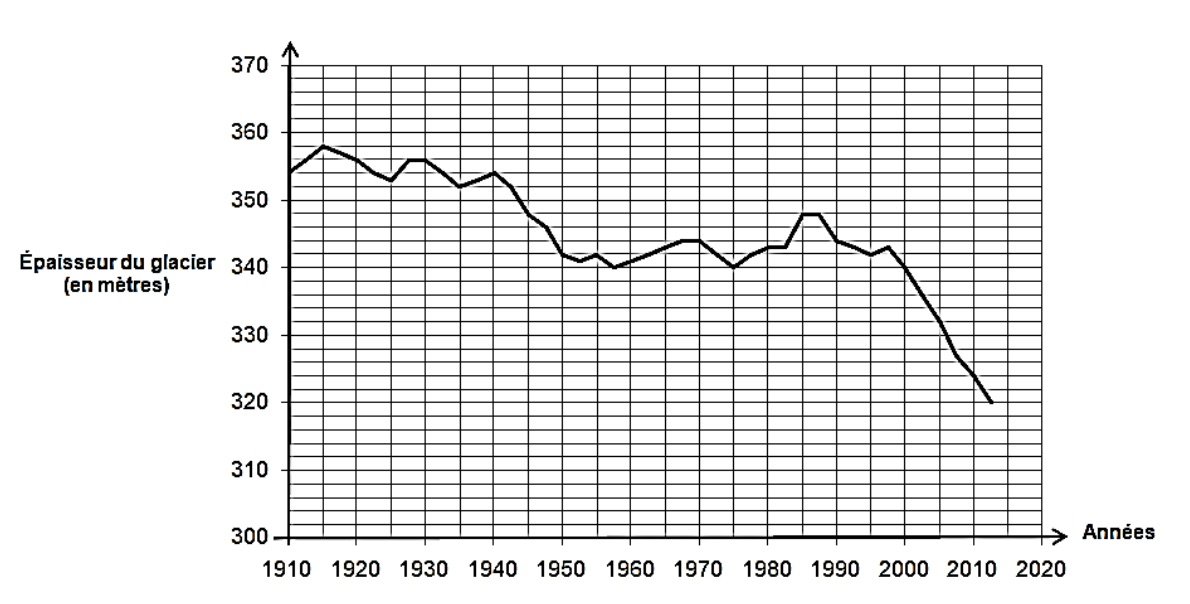
\includegraphics[width=1\linewidth]{img/brevet_blanc_01.jpg}
  \captionsetup{labelformat=empty}
  \caption{\label{} Doc 1 - Évolution au cours du temps de l'épaisseur en un point de la Mer de Glace (un
  glacier de montagne des Alpes)}
\end{figure} 

\begin{questions}
  \question[2] À l'aide du document ci-dessus, on montre que la diminution de l'épaisseur du glacier entre les années 1990 et 2000 est de 4 mètres. Déterminer la diminution de l'épaisseur du glacier entre les années 2000 et 2010. Justifier la réponse.
  \begin{solution}
    En 2000, l'épaisseur du glacier était de 340 mètres. En 2010, l'épaisseur du glacier était de 324 mètres. 
    La diminution de l'épaisseur du glacier s'exprime par la formule : 
    \[
    \delta = E_{2000} - E_{2010}
    \]
    où :
\begin{addmargin}[4em]{1em}
  \begin{compactitem}
      \item [$\delta$]: représente la différence d'épaisseur du glacier entre 2000 et 2010
      \item [$E_{2000}$]: représente l'épaisseur du glacier en 2000
      \item [$E_{2010}$]: représente l'épaisseur du glacier en 2010
  \end{compactitem}
\end{addmargin}
\textbf{Application numérique} : 
\[
    \delta = 340 - 324
  \]
  \[
    \delta = \SI{16}{m}
  \]
  L'épaisseur du glacier a diminué de 10 mètres entre 2000 et 2010.
  \end{solution}
  \question[2] Comparer les deux diminutions obtenues pour une durée de dix ans puis commenter. Quelle hypothèse peut-on formuler à propos du réchauffement climatique ?
  \begin{solution}
Entre 1990 et 2000, le glacier a perdu 4 mètres d'épaisseur \\
Entre 2000 et 2010, le glacier a perdu 16 mètres d'épaisseur. \\
Une comparaison peut se faire par calcul du rapport de fonte : 
\[
\alpha = \frac{\text{Fonte}_{2000 \text{ à } 2010}}{\text{Fonte}_{1990 \text{ à } 2000}}
\]

\textbf{Application numérique} : 
\[
  \frac{\text{Fonte}_{2000 \text{ à } 2010}}{\text{Fonte}_{1990 \text{ à } 2000}} = \frac{16}{4} = 4
  \]
donc
  \[
    {\text{Fonte}_{2000 \text{ à } 2010}} = 4 \times \text{Fonte}_{1990 \text{ à } 2000}
  \]
  Autrement dit, on peut dire que de 2000 à 2010, la fonte de l'épaisseur du glacier a été 4 fois plus importante qu'entre 1990 et 2000. On peut donc faire l'hypothèse que le réchauffement climatique s'est accéléré entre 2000 et 2010, par rapport à la période 1990-2000.
  \end{solution}
\end{questions}

\section*{Exercice 2 - Les fonds marins (6 points)}

\textit{Extrait du brevet 2024 - France Métropolitaine} \par

\subsection*{Les coraux}

Les coraux sont des êtres vivants marins dont le squelette est constitué de carbonate de calcium de formule chimique \ce{CaCO3}.

\begin{questions}
    \question[1] Indiquer le nombre d'atomes de carbone (\ce{C}) et le nombre d'atomes d'oxygène (\ce{O}) figurant dans la formule chimique du carbonate de calcium.
    \begin{solution}
      Il y a 1 atome de Carbone, et 3 atomes d'Oxygène. Attention, il ne fallait pas tomber dans le piège : \ce{Ca} représente un atome de calcium dans la molécule, et la question ne portait pas sur cet atome.
    \end{solution}
\end{questions}

\subsection*{L'environnement marin des coraux}

\textbf{Les ions sont simplement des atomes qui ont gagné ou perdu des électrons.} \par
\vspace{1em}
Le squelette des coraux contiennent des ions calcium \ce{Ca^2+} provenant de l'eau de mer.  
Afin de vérifier la présence de l'ion calcium \ce{Ca^2+} dans une eau de mer, on souhaite réaliser un test caractéristique sur un échantillon d'eau de mer.
On dispose des matériels et produits présentés dans le document 1 ci-dessous.

\begin{figure}[H]
  \centering
  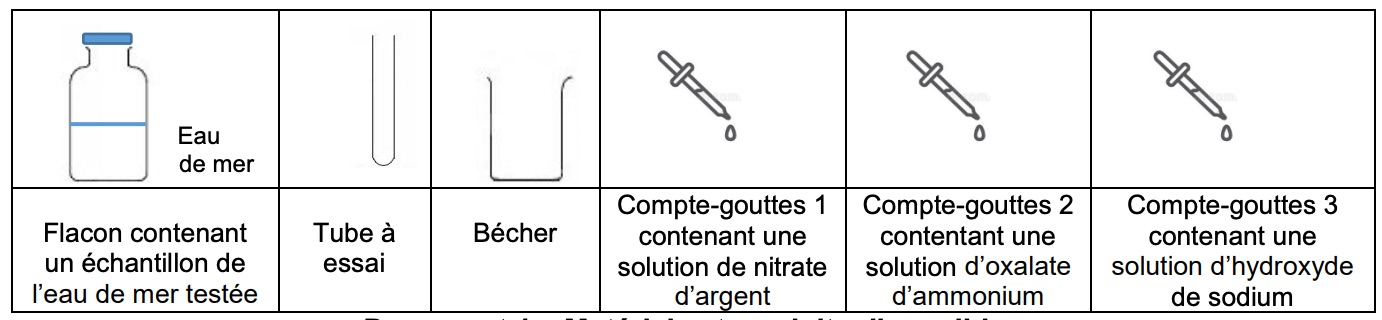
\includegraphics[width=0.9\linewidth]{img/brevet_blanc_02.jpg}
  \captionsetup{labelformat=empty}
  \caption{\label{} Doc 2 – Matériels et produits disponibles}
\end{figure} 

Le document 2 ci-après présente des tests caractéristiques de quelques ions.

\begin{figure}[H]
  \centering
  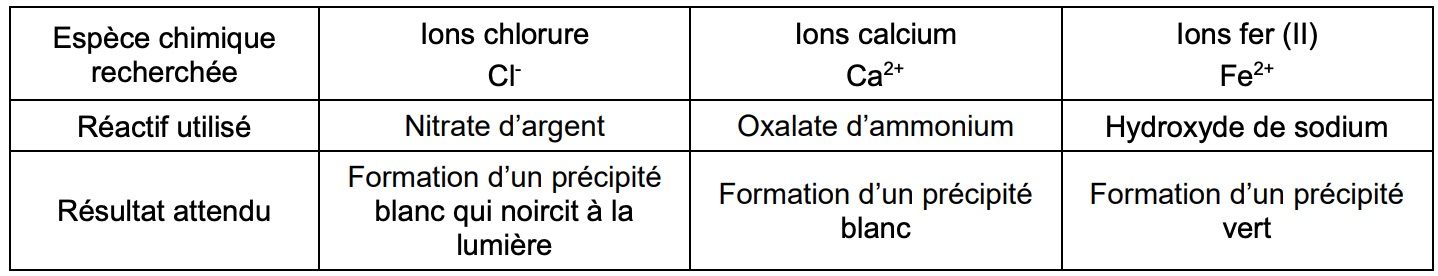
\includegraphics[width=0.8\linewidth]{img/brevet_blanc_03.jpg}
  \captionsetup{labelformat=empty}
  \caption{\label{} Doc 3 – Tests caractéristiques de quelques ions}
\end{figure} 

\begin{questions}
  \question[2] À l'aide des documents 2 et 3, proposer un protocole expérimental permettant de vérifier la présence de l'ion calcium \ce{Ca^2+} dans l'eau de mer testée. Les aspects liés à la sécurité ne sont pas attendus. \textbf{Remarque :} Il est possible de faire des schémas légendés.
  \begin{solution}
    \begin{itemize}
    \item On verse un peu d'eau de mer depuis le flacon vers le tube à essai. 
    \item On utilise le Compte-goutte 2 contenant la solution d'oxalate d'ammonium car c'est cette solution qui permet de détecter la présence d'ions calcium \ce{Ca^{2+}} (un précipité blanc est censé se former)
    \item On attend de voir si le réactif réagit avec l'eau de mer. Sinon, on peut jeter le mélange, laver le tube à essai. Et il pourra servir à un autre test pour tester la présence d'autres types d'ions.
    \item Il ne faut surtout pas mettre de goutte d'oxalate d'ammonium directement dans le flacon : sinon, on gache l'eau de mer. On veut pouvoir tester les réactifs et la présence d'ions un par un, indépendamment. 
    \end{itemize}
  \end{solution}
  \question[1] Dans l'expérience de la question précédente, indiquer l'observation attendue à l'issue du test si l'eau de mer contient des ions \ce{Ca^2+}.
  \begin{solution}
  On s'attend à ce qu'un précipité de couleur blanche se forme au moment où on ajoute les quelques gouttes d'oxalate d'ammonium.
  \end{solution}
\end{questions}

Pour déterminer la masse volumique d'une eau de mer, on réalise les mesures suivantes :

\begin{figure}[H]
  \centering
  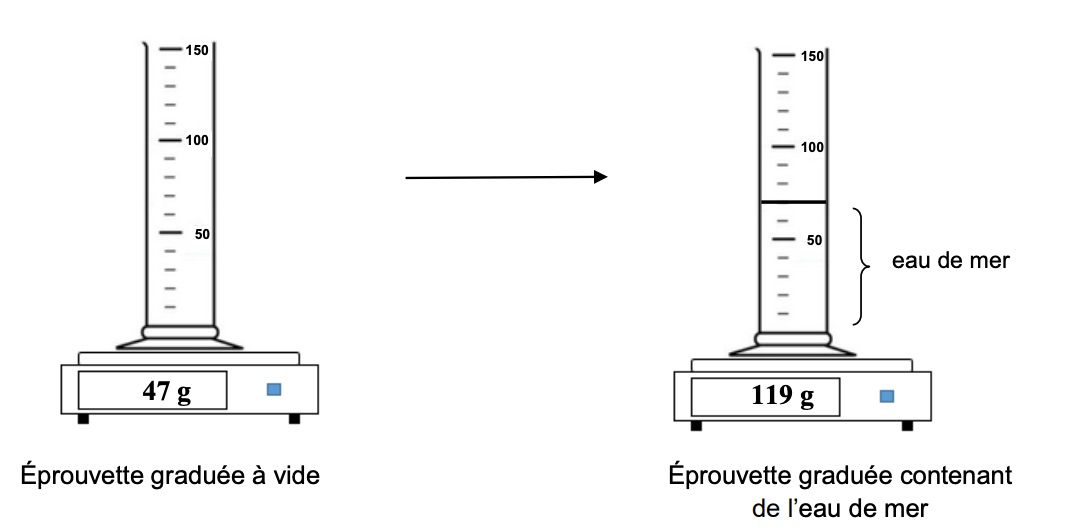
\includegraphics[width=0.9\linewidth]{img/brevet_blanc_04.jpg}
  \captionsetup{labelformat=empty}
  \caption{\label{} Doc 4 – Volumes et poids}
\end{figure} 

\textbf{L'éprouvette est graduée en millilitres (mL)}

\begin{questions}
  \question[2] À l'aide des résultats des mesures, déterminer la masse volumique de l'échantillon de l'eau de mer.
\end{questions}

\begin{solution}
  Pour déterminer la masse volumique de l'échantillon d'eau de mer, nous allons procéder comme suit :
  
  Données :
  \begin{itemize}[noitemsep]
    \item Masse de l'éprouvette vide : \( m_{\text{éprouvette}} = 47 \, \text{g} \),
    \item Masse de l'éprouvette remplie d'eau de mer : \( m_{\text{totale}} = 119 \, \text{g} \),
    \item Volume d'eau de mer dans l'éprouvette : \( V = 70 \, \text{mL} \).
  \end{itemize}
  
  1. Calcul de la masse de l'eau de mer
  La masse de l'eau de mer est donnée par :
  \[
  m_{\text{eau}} = m_{\text{totale}} - m_{\text{éprouvette}}
  \]
  Substitution des valeurs :
  \[
  m_{\text{eau}} = 119 \, \text{g} - 47 \, \text{g} = 72 \, \text{g}
  \]
  
  2. Calcul de la masse volumique 
  La masse volumique est donnée par la relation :
  \[
  \rho = \frac{m}{V}
  \]
  où :
  \begin{itemize}[noitemsep]
    \item \( m \) est la masse de l'eau (\( 72 \, \text{g} \)),
    \item \( V \) est le volume de l'eau (\( 70 \, \text{mL} \)).
  \end{itemize}
  
  Substitution des valeurs :
  \[
  \rho = \frac{72}{70} \approx 1,03 \, \text{g/mL}
  \]
  
  3. Conversion en unités SI (optionnel)
  Pour exprimer la masse volumique en unités SI :
  \[
  \rho = 1,03 \, \text{g/mL} = 1,03 \, \text{kg/L} = 1030 \, \text{kg/m}^3
  \]
  
  Conclusion :
  La masse volumique de l'échantillon d'eau de mer est :
  \[
  \rho = 1,03 \, \text{g/mL} \quad \text{ou} \quad \rho = 1030 \, \text{kg/m}^3
  \]
  
  Remarque :
  Il est important de bien lire les graduations de l'éprouvette. Dans ce cas, chaque graduation représente 10 mL, et non 2 mL, comme on peut le constater entre les marques 50 mL et 100 mL.
  \end{solution}

\section*{Exercice 3 - Déduction de formules (3 points)}

La formule de l'attraction gravitationnelle entre deux masses $m_1$ et $m_2$ est donnée par :

\[
F_g = G \cdot \frac{m_1 \cdot m_2}{r^2}
\]
où :
\begin{addmargin}[4em]{1em}
  \begin{compactitem}
      \item [$F_g$]: représente la force gravitationnelle (en newtons),
      \item [G]: représente la la constante gravitationnelle
      \item [$m_1$]: représente la masse du 1er corps.
      \item [$m_2$]: représente la masse du 2ème corps.
      \item [r]: représente a distance entre les deux corps (en mètres)
  \end{compactitem}
  \end{addmargin}


  \begin{questions}
    \question[3] Si dans un problème, je connais la valeur de la force gravitationnelle $F_g$, la constante gravitationnelle $G$, la masse $m_1$ et la distance entre les deux masses $r$. Comment peut-on déduire la masse $m_2$ ? \textbf{Une réponse sans justification vaudra 0 point. Si vous n'y arrivez pas sur ce sujet spécifique, vous pouvez prendre un autre exemple avec d'autres formules et comment vous pouvez vous en sortir avec une formule plus simple}
  
    \begin{solution}
      Pour déterminer la masse $m_2$, nous devons isoler cette grandeur dans l'équation donnée. Voici les étapes détaillées :
      
      \textbf{1. Partir de la formule de base :}
      \[
      F_g = G \cdot \frac{m_1 \cdot m_2}{r^2}
      \]
  
      \textbf{2. Réorganiser l'équation pour isoler $m_2$ :}
      On multiplie chaque membre de l'équation par $r^2$ pour se débarrasser du dénominateur :
      \[
      F_g \cdot r^2 = G \cdot m_1 \cdot m_2
      \]
  
      Ensuite, on divise chaque membre de l'équation par $G \cdot m_1$ pour isoler $m_2$ :
      \[
      m_2 = \frac{F_g \cdot r^2}{G \cdot m_1}
      \]
  
      \textbf{3. Vérifier les unités (optionnel) :}
      \begin{itemize}[noitemsep]
          \item $F_g$ est en newtons ($\text{N}$),
          \item $r$ est en mètres ($\text{m}$),
          \item $G$ est en $\text{N} \cdot \text{m}^2 \cdot \text{kg}^{-2}$,
          \item $m_1$ est en kilogrammes ($\text{kg}$).
      \end{itemize}
  
      L'unité de $m_2$ sera bien le kilogramme ($\text{kg}$).
  
      \textbf{4. Application numérique :}
      Si on connaît :
      \begin{itemize}[noitemsep]
          \item $F_g = 100$ N,
          \item $r = 10$ m,
          \item $G = 6,67 \times 10^{-11} \, \text{N} \cdot \text{m}^2 \cdot \text{kg}^{-2}$,
          \item $m_1 = 50$ kg,
      \end{itemize}
      alors, on applique les valeurs dans la formule :
      \[
      m_2 = \frac{100 \cdot (10)^2}{6,67 \times 10^{-11} \cdot 50}
      \]
  
      \textbf{5. Calcul détaillé :}
      \begin{align*}
      \text{Au numérateur :} & \quad 100 \cdot 10^2 = 100 \cdot 100 = 10\,000 \\
      \text{Au dénominateur :} & \quad 6,67 \cdot 10^{-11} \cdot 50 = 3,335 \cdot 10^{-9} \\
      \text{Division :} & \quad \frac{10\,000}{3,335 \cdot 10^{-9}} = 3,00 \times 10^{12}
      \end{align*}
  
      \textcolor{blue}{La masse $m_2$ est donc $3,00 \times 10^{12}$ kg.}
    \end{solution}
  \end{questions}

\end{document}
